\chapter{Cơ sở lý thuyết}
\label{chap2}

Hệ thống khuyến nghị là 1 công nghệ hỗ trợ đắc lực cho con người, 
giúp phân tích lượng dữ liệu khổng lồ được cung cấp bởi người dùng. 
Hệ thống dự đoán điểm của các sản phẩm, tạo 1 danh sách sắp xếp thứ các 
sản phẩm này cho mỗi người dùng, và giới thiệu tới người dùng những sản 
phẩm mà họ có thể thích. Nội dung trong phần này trình bày tổng quan về 
hệ khuyến nghị, các mô hình thuật toán cùng với các kỹ thuật thuật khai 
phá dữ liệu trong hệ khuyến nghị hiện có.
\begin{figure}[htbp]
    \centering
    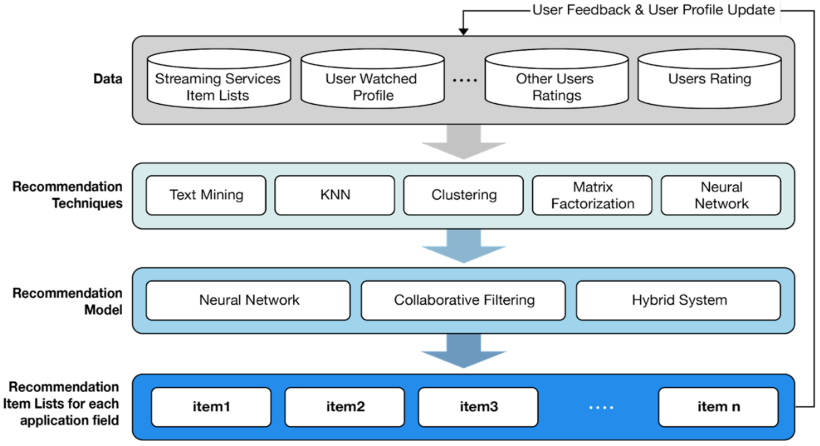
\includegraphics[width=1\textwidth]{imgs/chapter_2/tong-quan-htkn.png}
    \caption{Tổng quan hệ thống khuyến nghị}
    \label{tqhtkn}
\end{figure}
Hình \ref{tqhtkn} là tổng quan 
luồng hoạt động của 1 hệ khuyến nghị, gồm có các bước xử lý: (1) thu 
thập dữ liệu, (2) khai phá dữ liệu, (3) mô hình hóa dữ liệu, (4) và 
đưa ra gợi ý. Dữ liệu sử dụng trong hệ khuyến nghị có thể là các đánh 
giá, bình luận về sản phẩm, danh sách sản phẩm mà người dùng theo dõi, 
v.v. Các kỹ thuật khai phá dữ liệu truyền thống, có thể kể đến như: 
phân cụm, khai phá dữ liệu văn bản, KNN hay là học sâu, sử dụng mạng 
nơ-ron. Tiếp đó, các mô hình khuyến nghị sử dụng các đặc trưng đã 
được trích chọn để có thể mô hình hóa dữ liệu, từ đó đưa ra các khuyến 
nghị phù hợp tới người dùng.

Nội dung trong chương này tập trung giới thiệu và phân loại một cách tổng 
quát về các mô hình khuyến nghị hiện nay, có thể áp dụng vào bất kỳ 1 hệ thống khuyến
nghị nào.

\section{Phân loại mô hình khuyến nghị}
Các mô hình khuyến nghị có thể được chia thành 3 nhóm chính \cite{goyani2020review}:
\begin{itemize}
    \item \textbf{Lọc dựa trên nội dung}: Trong cách tiếp cận này, hệ thống sẽ thu thập các dữ
    liệu rõ ràng (điểm đánh giá sản phẩm) hoặc dữ liệu ngầm (bấm vào một đường
    dẫn) và tạo ra hồ sơ người dùng. Hệ thống sẽ thực hiện tư vấn những sản phẩm
    dựa trên những sản phẩm và hành vi liên quan tới hồ sơ người dùng. Do sở thích 
    của người dùng thường được chia thành vài nhóm cơ bản, việc chỉ sử dụng hồ sơ
    của 1 người dùng khiến hệ thống không tận dụng được thông tin từ những người
    dùng khác, từ đó hạn chế sự linh hoạt của hệ tư vấn.

    \item \textbf{Lọc cộng tác}: Không giống với lọc dựa trên nội dung, lọc cộng tác tìm kiếm
    những người dùng có sở thích tương tự nhau. Từ giả định những người dùng A
    có sở thích giống với người dùng B, hệ thống sẽ tiến hành tư vấn cho người dùng
    B những sản phẩm phù hợp người dùng A. Lọc cộng tác có 2 hướng tiếp cận: dựa
    trên bộ nhớ và dựa trên mô hình. Hướng tiếp cận dựa trên bộ nhớ tính toán độ
    tương tự giữa các người dùng từ đó thực hiện tư vấn. Nhược điểm của hướng tiếp
    cận này là sự tốn kém tài nguyên khi số lượng người dùng và sản phẩm tăng lên.
    Hướng tiếp cận dựa trên mô hình sử dụng các mô hình đã được huấn luyện thông
    qua các thuật toán học máy hoặc khai phá dữ liệu để thực hiện tư vấn.

    \item \textbf{Hệ tư vấn lai} Lọc dựa trên nội dung và lọc cộng tác đều có ưu điểm và nhược
    điểm riêng. Để giải quyết vấn đề này, hệ tư vấn lai được sinh ra, là sự kết hợp
    của 2 kỹ thuật trên.
\end{itemize}

Trong phần tiếp theo, đồ án sẽ tập trung vào việc trình bày mô hình 1 số lọc cộng
tác tiêu biểu.

\section{Lọc cộng tác}
Lọc cộng tác là một mô hình lọc thông tin, xây dựng 1 cơ sở dữ liệu sở thích người dùng 
thông qua dữ liệu tưởng tác giữa họ với sản phẩm để dự đoán các sản phẩm phù hợp với sở thích của họ, 
từ đó đưa ra các khuyến nghị về sản phẩm. Ý tưởng của mô hình lọc cộng tác là từ dữ liệu hành vi
tương tác giữa người dùng và sản phẩm, hệ thống sẽ tính toán mức độ tương đồng giữa các người dùng
hoặc giữa các sản phẩm, tạo cơ sở thực hiện khuyến nghị. Những người dùng có mức độ tương đồng cao
sẽ có xu hướng mua những sản phẩm giống nhau. Với mỗi cách tính độ tương đồng sẽ cho một mô hình lọc cộng tác 
khác nhau.

Các mô hình lọc cộng tác có thể được chia ra thông qua 2 hướng tiếp cận: lọc cộng tác dựa trên bộ nhớ và 
lọc cộng tác dựa trên mô hình. Hướng tiếp cận dựa trên bộ nhớ tính toán độ
tương tự giữa các người dùng từ đó thực hiện tư vấn. Nhược điểm của hướng tiếp
cận này là sự tốn kém tài nguyên khi số lượng người dùng và sản phẩm tăng lên. Ngoài ra, hệ 
thống cần tính toán tại thời điểm khuyến nghị, điều này sẽ ảnh hưởng tới thời gian đưa ra dự đoán.
Hướng tiếp cận dựa trên mô hình sử dụng các mô hình đã được huấn luyện thông
qua các thuật toán học máy hoặc khai phá dữ liệu để thực hiện tư vấn. Với hướng tiếp cận này, 
mô hình sẽ cần phải thực hiện huấn luyện trước, nhưng khi thực hiện khuyến nghị sẽ rất nhanh. 
Trong lọc cộng tác dựa trên bộ nhớ, ta có thể phân loại thành: 
lọc cộng tác dựa trên người dùng và lọc cộng tác dựa trên sản phẩm. Lọc cộng tác dựa trên người dùng là 
1 mô hình so sánh sự tương đồng giữa các người dùng thông qua dữ liệu tương tác của họ lên 
các sản phẩm, từ đó khuyến nghị các sản phẩm phù hợp. Lọc cộng tác dựa trên sản phẩm dự 
đoán bằng cách sử dụng độ tương đồng giữa sản phẩm và sản phẩm được chọn bởi người dùng 
thông qua 1 ma trận tương tác của người dùng và sản phẩm. Nói cách khác, lọc cộng tác dựa 
trên bộ nhớ sử dụng các kỹ thuật như: độ tương quan Pearson, độ tương quan cô-sin, KNN 
để tạo các nhóm có đặc tính giống nhau, từ đó khuyến nghị các sản phẩm tới người dùng trong 
nhóm. Do cách hoạt động dựa trên dữ liệu đánh giá, nên mô hình khó có thể hoạt động tốt 
khi không có đủ dữ liệu cần thiết. Để khắc phục vấn đề này, lọc cộng tác dựa trên mô hình 
đưa ra khuyến nghị nhờ sử dụng các thuật toán như: phân cụm, SVD hay PCA.

\subsection{Lọc cộng tác dựa trên bộ nhớ}

\begin{figure}[htbp]
    \centering
    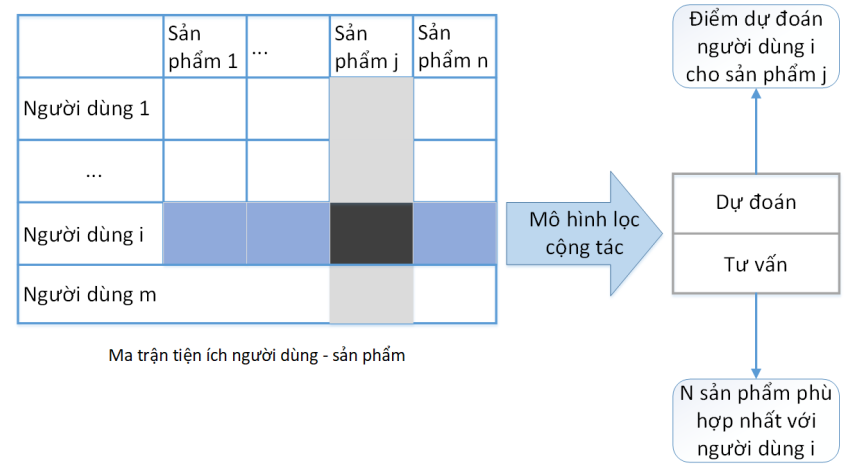
\includegraphics[width=1\textwidth]{imgs/chapter_2/loc-cong-tac.png}
    \caption{Mô hình thuật toán lọc cộng tác}
    \label{lct}
\end{figure}
Thông thường, hồ sơ người dùng – sản phẩm thường được xây dựng từ điểm đánh giá người dùng chấm
cho sản phẩm, được gọi là ma trận tương tác. Ma trận tương tác sẽ có dạng như trong Hình \ref{lct}, với các hàng/cột là danh sách người dùng, cột/hàng là danh sách sản phẩm, các giá
trị trong mỗi ô tương ứng với điểm đánh giá người dùng danh cho sản phẩm. Trong thực
tế, người dùng thường ít đánh giá sản phẩm nên ma trận tiện ích trở nên thưa thớt, nghĩa
là có nhiều giá trị chưa được điền. Hình \ref{lct} là mô hình xử lý, mô tả cho thuật toán lọc
cộng, tác được chia thành 3 bước thực hiện:
\begin{enumerate}
    \item Chuẩn hóa dữ liệu
    \item Tính toán độ tương đồng
    \item Dự đoán mức độ quan tâm của người dùng lên sản phẩm
\end{enumerate}

\subsubsection{Lọc cộng tác dựa trên người dùng}

\underline{Bước 1: Chuẩn hóa dữ liệu}

    Trong thực tế, người dùng “lười” đánh giá sản phẩm khiến ma trận tiện ích trở nên
thưa thớt. Do đó cần chuẩn hóa dữ liệu để loại bỏ những giá trị chưa biết trong ma trận.
Xét ví dụ trong Bảng 1.1 là ma trận tiện ích được xây dựng từ tập người dùng $W = {w_1, ..., w_5}$ và tập sản phẩm $X={x_1, ..., x_5}$. Mỗi sản phẩm được người dùng đánh giá trên thang điểm từ 0 đến 5. Các giá trị “?” nghĩa là người dùng chưa đánh giá những sản phẩm tương ứng.

\begin{table}[h]
\centering
\begin{tabularx}{\textwidth}{|l|>{\centering\arraybackslash}X|>{\centering\arraybackslash}X|>{\centering\arraybackslash}X|>{\centering\arraybackslash}X|>{\centering\arraybackslash}X|}
\hline
      & $x_1$ & $x_2$ & $x_3$ & $x_4$ & $x_5$ \\ \hline
$w_1$ & 5     & 5     & 2     & 0     & ?     \\ \hline
$w_2$ & 2     & 4     & 0     & ?     & ?     \\ \hline
$w_3$ & 0     & 1     & 3     & 4     & 5     \\ \hline
$w_4$ & 5     & ?     & ?     & ?     & 1     \\ \hline
$w_5$ & ?     & ?     & 3     & 2     & 4     \\ \hline
\end{tabularx}
\caption{Ví dụ ma trận tương tác}
\end{table}

    Cách dễ nhất để điền các giá trị còn thiếu vào trong ma trận này là chọn điểm cao nhất
hoặc điểm thấp nhất (5 hoặc 0). Tuy nhiên, khi chọn giá trị này sẽ gây mất cân bằng và
giảm độ chính xác của hệ thống. Một giá trị an toàn có thể điển là điểm trung bình của
thang đo (2,5). Tuy nhiên, giá trị này sẽ không đúng với những người dùng khó tính
hoặc dễ tính. Vì người dùng khó tính sẽ chỉ cho 4 với những sản phẩm họ thích, ngược
lại người dùng dễ tính sẽ cho 1, 2 với những sản phẩm họ không thích. Do đó cần có
một cách chuẩn hóa khác để khắc phục vấn đề này. Các bước chuẩn hóa sẽ được trình bày ngay sau đây. 
\begin{enumerate}
    \item Tính trung bình các điểm đánh giá mà mỗi người dùng đã đưa ra. Ví dụ, người dùng
    $w_1$ đã chấm 4 sản phẩm với số điểm lần lượt là: 5, 5, 2, 0. Như vậy, điểm trung bình người dùng $w_1$ đưa ra là: $\frac{5+5+2+0}{4}=3$.
    \begin{table}[h]
    \centering
    \begin{tabularx}{\textwidth}{|l|>{\centering\arraybackslash}X|>{\centering\arraybackslash}X|>{\centering\arraybackslash}X|>{\centering\arraybackslash}X|>{\centering\arraybackslash}X|
    >{\centering\arraybackslash}X|}
    \hline
          & $x_1$ & $x_2$ & $x_3$ & $x_4$ & $x_5$ & Điểm TB \\ \hline
    $w_1$ & 5     & 5     & 2     & 0     & ?     & 3 \\ \hline
    $w_2$ & 2     & 4     & 0     & ?     & ?     & 2 \\ \hline
    $w_3$ & 0     & 1     & 3     & 4     & 5     & 2.6 \\ \hline
    $w_4$ & 5     & ?     & ?     & ?     & 1     & 3 \\ \hline
    $w_5$ & ?     & ?     & 3     & 2     & 4     & 3 \\ \hline
    \end{tabularx}
    \caption{Ví dụ ma trận tương tác}
    \end{table}

    \item Thực hiện trừ điểm đánh giá của người dùng với điểm đánh giá trung bình của họ
    \begin{table}[h]
    \centering
    \begin{tabularx}{\textwidth}{|l|>{\centering\arraybackslash}X|>{\centering\arraybackslash}X|>{\centering\arraybackslash}X|>{\centering\arraybackslash}X|>{\centering\arraybackslash}X|
    >{\centering\arraybackslash}X|}
    \hline
          & $x_1$ & $x_2$ & $x_3$ & $x_4$ & $x_5$ & Điểm TB \\ \hline
    $w_1$ & 2     & 2     & -1    & -3    & ?     & 3 \\ \hline
    $w_2$ & 0     & 2     & -2    & ?     & ?     & 2 \\ \hline
    $w_3$ & -2.6  & -1.6  & 0.4   & 1.4   & 2.4     & 2.6 \\ \hline
    $w_4$ & 2     & ?     & ?     & ?     & -2     & 3 \\ \hline
    $w_5$ & ?     & ?     & 0     & -1    & 1     & 3 \\ \hline
    \end{tabularx}
    \caption{Ví dụ ma trận tương tác}
    \end{table}

    \item Các ô chưa biết thì điền 0.
    \begin{table}[h]
    \centering
    \begin{tabularx}{\textwidth}{|l|>{\centering\arraybackslash}X|>{\centering\arraybackslash}X|>{\centering\arraybackslash}X|>{\centering\arraybackslash}X|>{\centering\arraybackslash}X|
    >{\centering\arraybackslash}X|}
    \hline
          & $x_1$ & $x_2$ & $x_3$ & $x_4$ & $x_5$ & Điểm TB \\ \hline
    $w_1$ & 2     & 2     & -1    & -3    & 0     & 3 \\ \hline
    $w_2$ & 0     & 2     & -2    & ?     & 0     & 2 \\ \hline
    $w_3$ & -2.6  & -1.6  & 0.4   & 1.4   & 2.4     & 2.6 \\ \hline
    $w_4$ & 2     & 0     & 0     & 0     & -2     & 3 \\ \hline
    $w_5$ & 0     & 0     & 0     & -1    & 1     & 3 \\ \hline
    \end{tabularx}
    \caption{Ví dụ ma trận tương tác}
    \end{table}
\end{enumerate}

Cách chuẩn hóa trên có 2 ưu điểm: (1) Việc trừ đi điểm đánh giá trung bình của người dùng khiến ma trận có giá trị âm, dương. Những giá trị dương ứng với những sản phẩm được người dùng quan tâm
hơn. Những ô có giá trị 0 biểu diễn cho người dùng chưa đánh giá sản phẩm này. Đây là những giá trị cần dự đoán. (2) Số chiều của ma trận tiện ích là rất lớn khi người dùng và sản phẩm tăng lên. Vì vậy, để tiết kiệm bộ nhớ, ma trận tiện ích sẽ được lưu dưới dạng ma trận thưa do những dấu “?” đã được thay bằng giá trị 0.

\underline{Bước 2: Tính toán độ tương đồng và dự đoán}

Với mỗi cách tính độ tương đồng sẽ cho ra một thuật toán lọc cộng tác khác nhau.
Nếu tính độ tương đồng giữa các cặp người dùng ta có thuật toán lọc cộng tác người
dùng. Nếu tính độ tương đồng giữa các cặp sản phẩm, ta có thuật toán lọc cộng tác sản
phẩm. Để tính độ tương đồng giữa người dùng $w_i$ và $w_j$ , ta sử dụng công thức cô-sin:
\begin{equation}
    cosin\_similarity(w_i, w_j) = cos(w_i, w_j)=\frac{w_i^T w_j}{||w_i||_2||w_j||_2}
\end{equation}
Trong đó, $w_i$ và $w_j$ là các véc-tơ tương ứng với hàng/cột $w_i$ và $w_j$ trong ma trận tương tác. Sau khi tính toán được độ tương đồng giữa các cặp người dùng, thuật toán sẽ dự đoán
mức độ quan tâm của người dùng $u$ lên sản phẩm $i$ dựa trên thông tin từ K người dùng
giống $u$ nhất, được định nghĩa theo công thức:
\begin{equation}
    \hat{y}_{i,u}=\frac{\sum_{u, j \in \mathrm{N}(u,i)} \bar{y}_{i, u_j}sim(u, u_j)}{\sum_{u, j \in \mathrm{N}(u,i)}|sim(u,u_j)|}
\end{equation}
Với $N(u,i)$ là tập hợp K người dùng gần giống $u$ nhất và đã đánh giá sản phẩm $i$.

Lọc cộng tác người dùng thường hoạt động không hiệu quả trên các hệ thống lớn do số lượng người dùng khổng lồ. Khi đó, việc tính toán độ tương đồng giữa các cặp người dùng trở nên tốn kém tài nguyên là thời gian.

\subsubsection{Lọc cộng tác dựa trên sản phẩm}
Lọc cộng tác sản phẩm là hướng tiếp cận có thể khắc phục nhược điểm của lọc cộng tác người dùng do số lượng sản phẩm trên hệ thống thường không biến động mạnh. Thay vì tính toán độ tương động giữa các cặp người dùng, lọc cộng tác sản phẩm tính toán độ tương đồng giữa các sản phẩm.

\underline{Chuẩn hóa dữ liệu}
\begin{itemize}
    \item Tính trung bình điểm đánh giá sản phẩm nhận được
    \begin{table}[h]
        \centering
        \begin{tabularx}{\textwidth}{|l|>{\centering\arraybackslash}X|>{\centering\arraybackslash}X|>{\centering\arraybackslash}X|>{\centering\arraybackslash}X|>{\centering\arraybackslash}X|
        >{\centering\arraybackslash}X|}
        \hline
                & $x_1$ & $x_2$ & $x_3$ & $x_4$ & $x_5$ \\ \hline
        $w_1$ & 5     & 5     & 2     & 0     & ?     \\ \hline
        $w_2$ & 2     & 4     & 0     & ?     & ?     \\ \hline
        $w_3$ & 0     & 1     & 3     & 4     & 5     \\ \hline
        $w_4$ & 5     & ?     & ?     & ?     & 1     \\ \hline
        $w_5$ & ?     & ?     & 3     & 2     & 4     \\ \hline
        Điểm TB & 3 & 3.333 & 2 & 2 & 3.333\\ \hline
        \end{tabularx}
        \caption{Ví dụ ma trận tương tác}
    \end{table}

    \item Thực hiện trừ điểm đánh giá của sản phẩm với điểm đánh giá trung bình
    \begin{table}[h]
        \centering
        \begin{tabularx}{\textwidth}{|l|>{\centering\arraybackslash}X|>{\centering\arraybackslash}X|>{\centering\arraybackslash}X|>{\centering\arraybackslash}X|>{\centering\arraybackslash}X|
        >{\centering\arraybackslash}X|}
        \hline
                & $x_1$ & $x_2$ & $x_3$ & $x_4$ & $x_5$ \\ \hline
        $w_1$ & 2     & 1.667 & 0     & -2     & ?       \\ \hline
        $w_2$ & -1    & 0.667 & -2     & ?     & ?      \\ \hline
        $w_3$ & -3    & -2.333& 1     & 2     & 1.667       \\ \hline
        $w_4$ & 2     & ?     & ?     & ?     & -2.333       \\ \hline
        $w_5$ & ?     & ?     & 1     & 0     & 0.667       \\ \hline
        Điểm TB & 3   & 3.333 & 2     & 2     & 3.333   \\ \hline
        \end{tabularx}
        \caption{Ví dụ ma trận tương tác}
    \end{table}

    \item Các ô "?" điền giá trị 0
    \begin{table}[h]
        \centering
        \begin{tabularx}{\textwidth}{|l|>{\centering\arraybackslash}X|>{\centering\arraybackslash}X|>{\centering\arraybackslash}X|>{\centering\arraybackslash}X|>{\centering\arraybackslash}X|
        >{\centering\arraybackslash}X|}
        \hline
                & $x_1$ & $x_2$ & $x_3$ & $x_4$ & $x_5$ \\ \hline
        $w_1$ & 2     & 1.667 & 0     & -2     & 0       \\ \hline
        $w_2$ & -1    & 0.667 & -2     & 0     & 0      \\ \hline
        $w_3$ & -3    & -2.333& 1     & 2     & 1.667       \\ \hline
        $w_4$ & 2     & 0     & 0     & 0     & -2.333       \\ \hline
        $w_5$ & 0     & 0     & 1     & 0     & 0.667       \\ \hline
        Điểm TB & 3   & 3.333 & 2     & 2     & 3.333   \\ \hline
        \end{tabularx}
        \caption{Ví dụ ma trận tương tác}
    \end{table}
\end{itemize}

\underline{Tính toán độ tương đồng và dự đoán}

Dự đoán độ quan tâm của $w_2$ lên $w_5$ sử dụng lọc cộng tác sản phẩm.
\begin{itemize}
    \item Sản phẩm được $w_2$ đánh giá: $\{x_1, x_2, x_3\}$
    \item Độ tương tự giữa $x_5$ và $\{x_1, x_2, x_3\}$ lần lượt là: \{-0.774, -0.449, 0.324\}
    \item Xét K=2, ta có 2 sản phẩm giống $x_5$ nhất : $N(u,i) = \{x_2, x_3\}$ với 
    điểm đánh giá chuẩn hóa là \{0.667, -2\}
    \item $\hat{y}_{(w_2, x_5)}=\frac{0.667*-0.449+(-2)*0.324}{0.324+|-0.449|}=-1.226$
    \item Đưa điểm đánh giá về thang đo ban đầu, ta cộng điểm đánh giá dự đoán với điểm đánh giá
            trung bình của sản phẩm: $-1.226+3.333=2.107$
\end{itemize}

\subsection{Lọc cộng tác phân tích ma trận}
\subsubsection{Giới thiệu}
Ý tưởng chính của phương pháp này là tồn tại các đặc trưng ẩn mô tả sự liên quan
giữa các sản phẩm và người dùng. Ví dụ với các bộ phim, các đặc trưng ẩn có thể rõ 
ràng như: hài, chính kịch, hành động, hoặc chúng là sự kết hợp của các đặc trưng ẩn rõ
ràng, hoặc chúng là những đặc trưng chưa được đặt tên. Tương tự, mỗi người dùng cũng
sẽ có xu hướng thích những đặc trưng ẩn nào đó của phim. Thay vì xây dựng ma trận
của $M$ sản phẩm $X$ một cách độc lập, các đặc trưng ẩn này được huấn luyện đồng thời
với dữ liệu của ma trận $N$ người dùng $Y$.

Với ý tưởng trên, thay vì xây dựng ma trận $Y$ nghĩa là dự đoán các giá trị còn khuyết
trong $Y$ thì thuật toán sẽ cố gắng sấp xỉ ma trận người dùng $W$ và ma trận sản phẩm $X$,
sao cho tích của 2 ma trận này là $\hat{Y}$ xấp xỉ với $Y$.
$$Y \approx \hat{Y} = X^TW$$